%!TEX TS-program = xelatex
%!TEX encoding = UTF-8 Unicode

% Author: Romain "Artefact2" Dal Maso <artefact2@gmail.com>
% 
% This program is free software. It comes without any warranty, to the
% extent permitted by applicable law. You can redistribute it and/or
% modify it under the terms of the Do What The Fuck You Want To Public
% License, Version 2, as published by Sam Hocevar. See
% http://sam.zoy.org/wtfpl/COPYING for more details.

\newlength{\hbArtRealHeight}
\newlength{\hbArtFakeHeight}
\newlength{\hbArtFakeHeightHack}

% XXX why the 1pt offset?
\newlength{\hbArtLeftOffset}
\setlength{\hbArtLeftOffset}{\maxof{\foremargin}{\spinemargin}+1pt}
\newlength{\hbArtOvershootWidth}
\setlength{\hbArtOvershootWidth}{\maxof{\foremargin}{\spinemargin}-\minof{\foremargin}{\spinemargin}+2pt}
\newlength{\hbArtTopOffset}
\setlength{\hbArtTopOffset}{\uppermargin}
\newlength{\hbArtBottomOffset}
\setlength{\hbArtBottomOffset}{\paperheight-\uppermargin-\textheight}

% XXX is it wise to use floats for this? they have a LOT of issues. Is
% it possible to alter the margins of the CURRENT page?  Look into
% geometry (inserts \clearpage, not good) and/or changepage (nope,
% doesn't work with memoir it seems?)

% XXX: left margin is wrong half the time, we need to overshoot

% Real W/H ratio (per the picture spec), fictional W/H ratio (wrt margins), Filename
\newcommand*{\hbWideBottomArt}[3]{%
  \FPeval{\result}{1/#1}%
  \setlength{\hbArtRealHeight}{\result\paperwidth}%
  \FPeval{\result}{1/#2}%
  \setlength{\hbArtFakeHeight}{\result\paperwidth}%
  \begin{figure*}[!b]%
    % XXX 1pt offset?
    \begin{rtb*}{\paperwidth+\hbArtOvershootWidth}{-\hbArtLeftOffset}{\hbArtFakeHeight-\hbArtRealHeight}%
      \includegraphics[width=\paperwidth+\hbArtOvershootWidth,height=\hbArtRealHeight]{#3}
    \end{rtb*}%
    \rule{0pt}{\maxof{0pt}{\hbArtFakeHeight-\hbArtBottomOffset}}%
  \end{figure*}%
}

\newcommand*{\hbWideTopArt}[3]{%
  \FPeval{\result}{1/#1}%
  \setlength{\hbArtRealHeight}{\result\paperwidth}%
  \FPeval{\result}{1/#2}%
  \setlength{\hbArtFakeHeight}{\result\paperwidth}%
  \begin{figure*}[!t]%
    \begin{rtb*}{\paperwidth+\hbArtOvershootWidth}{-\hbArtLeftOffset}{-\hbArtTopOffset}%
      \includegraphics[width=\paperwidth+\hbArtOvershootWidth,height=\hbArtRealHeight]{#3}
    \end{rtb*}%
    \rule{0pt}{\maxof{0pt}{\hbArtFakeHeight-\hbArtTopOffset}}%
  \end{figure*}%
}

% XXX: https://tug.org/TUGboat/tb35-3/tb111beet-banner.pdf
% It's ugly and limited, but also the best TeX can do
\newcommand*{\hbWideBottomArtFirstPageFix}{}
\newcommand*{\hbWideBottomArtFirstPage}[3]{%
  \FPeval{\result}{1/#1}%
  \setlength{\hbArtRealHeight}{\result\paperwidth}%
  \FPeval{\result}{1/#2}%
  \setlength{\hbArtFakeHeight}{\result\paperwidth}%
  \setlength{\hbArtFakeHeightHack}{\maxof{0pt}{\hbArtFakeHeight-\hbArtBottomOffset}}%
  \renewcommand*{\hbWideBottomArtFirstPageFix}{\enlargethispage{-\hbArtFakeHeightHack}}%
  \begin{figure}[!b]%
    \begin{rtb*}{\paperwidth+\hbArtOvershootWidth}{-\hbArtLeftOffset}{\hbArtFakeHeight-\hbArtRealHeight}%
      \includegraphics[width=\paperwidth+\hbArtOvershootWidth,height=\hbArtRealHeight]{#3}
    \end{rtb*}%
    \rule{0pt}{\hbArtFakeHeightHack}%
  \end{figure}%
}

\newcommand*{\hbFullPageArt}[1]{%
  \clearpage%
  \AddThispageHook{%
    \begin{tb*}{\paperwidth}{0pt}{0pt}%
      \includegraphics[width=\paperwidth,height=\paperheight]{#1}
    \end{tb*}%
    \begin{tb*}{\paperwidth}{0pt}{0pt}%
      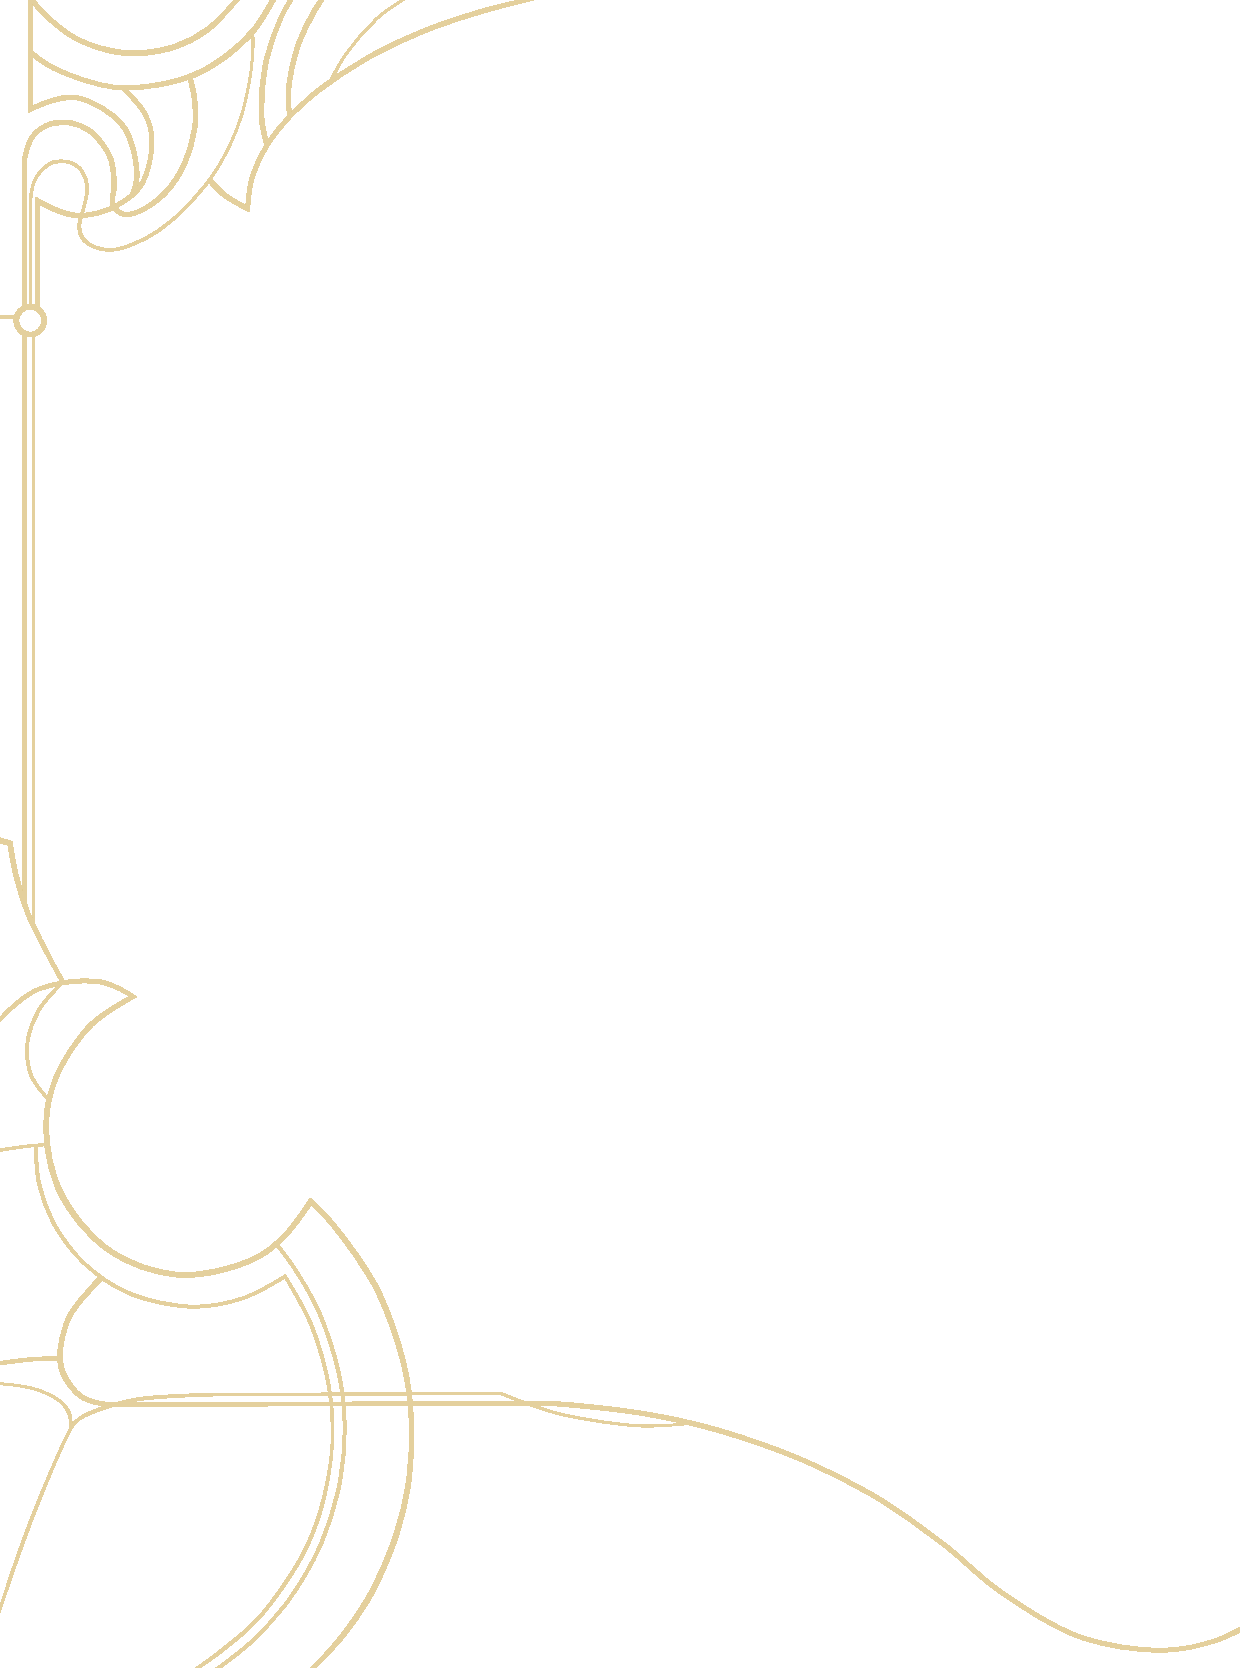
\includegraphics[width=\paperwidth,height=\paperheight]{assets/full-page-decoration}
    \end{tb*}%
  }%
  \clearpage%
}
